\section{SimSite3D::dir\_\-point\_\-t Class Reference}
\label{classSimSite3D_1_1dir__point__t}\index{SimSite3D::dir_point_t@{SimSite3D::dir\_\-point\_\-t}}
A point and associated direction.  


{\tt \#include $<$dir\_\-point.H$>$}

Inheritance diagram for SimSite3D::dir\_\-point\_\-t::\begin{figure}[H]
\begin{center}
\leavevmode
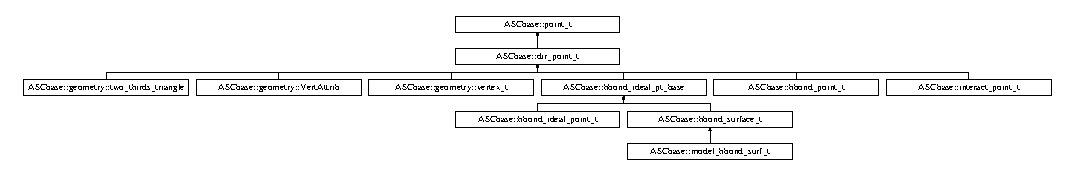
\includegraphics[height=1.92044cm]{classSimSite3D_1_1dir__point__t}
\end{center}
\end{figure}
\subsection*{Public Member Functions}
\begin{CompactItemize}
\item 
\textbf{dir\_\-point\_\-t} (alloc\_\-t a=ALLOC\_\-POSITION)\label{classSimSite3D_1_1dir__point__t_57018723a8991fa7f47cc485ba6f3d86}

\item 
\textbf{dir\_\-point\_\-t} (const \bf{dir\_\-point\_\-t} \&p)\label{classSimSite3D_1_1dir__point__t_3931e2347f2aee30a6d72ccdb211c7bb}

\item 
const \bf{dir\_\-point\_\-t} \& \textbf{operator=} (const \bf{dir\_\-point\_\-t} \&p)\label{classSimSite3D_1_1dir__point__t_b45b7d7b83e413955ac14b3ccf2336c4}

\item 
void \textbf{delete\_\-dir} ()\label{classSimSite3D_1_1dir__point__t_dfb4e224f9037f3e14101f5098d5a6c8}

\end{CompactItemize}
\subsection*{Public Attributes}
\begin{CompactItemize}
\item 
my\_\-float\_\-t $\ast$ \textbf{dir}\label{classSimSite3D_1_1dir__point__t_7378ba825067f07353f214941ca4a715}

\end{CompactItemize}
\subsection*{Private Member Functions}
\begin{CompactItemize}
\item 
void \textbf{do\_\-copy} (const \bf{dir\_\-point\_\-t} \&p)\label{classSimSite3D_1_1dir__point__t_80fca05c410b767d5eff066f3e5708bd}

\end{CompactItemize}
\subsection*{Private Attributes}
\begin{CompactItemize}
\item 
alloc\_\-t \textbf{\_\-dir\_\-allocated}\label{classSimSite3D_1_1dir__point__t_14646e021c9e24eedf8a41ef4f6dc68d}

\end{CompactItemize}


\subsection{Detailed Description}
A point and associated direction. 



The documentation for this class was generated from the following file:\begin{CompactItemize}
\item 
dir\_\-point.H\end{CompactItemize}
